\documentclass{ctexart}
\usepackage[T1]{fontenc}
\usepackage[a4paper,top=1.5cm,bottom=1.5cm,left=2cm,right=2cm,marginparwidth=1.75cm]{geometry}
\usepackage{mathtools}
\usepackage{tikz}
\usepackage{booktabs}
\usepackage{caption}
\usepackage{outlines}
\usepackage{graphicx}
\usepackage{minted}
\usepackage{amsthm}
\usepackage[colorlinks=false, allcolors=blue]{hyperref}
\renewcommand{\tableautorefname}{表}
\DeclarePairedDelimiter{\set}{\{}{\}}
\DeclarePairedDelimiter{\paren}{(}{)}
\graphicspath{ {./images/} }

\title{微机接口第五次作业}
\author{卢雨轩 19071125}
% \date{\today}
\ctexset{
    section = {
        titleformat = \raggedright,
        name = {,},
        number = \chinese{section}、
    },
    paragraph = {
        runin = false
    },
    today = small,
    figurename = 图,
    contentsname = 目录,
    tablename = 表,
}

\begin{document}

\maketitle

\begin{outline}[enumerate]
    \1 设8253的通道0-2和控制端口的地址分别为300H、302H、304H和306H,定义通道0工作在方式3,CLK0=2MHz。试编写初始化程序,并画出硬件连线图。要求通道0输出1.5kHz的方波,通道1用通道0的输出作计数脉冲,输出频率为300Hz的序列负脉冲,通道2每秒钟向CPU发50次中断请求。

    \begin{center}
        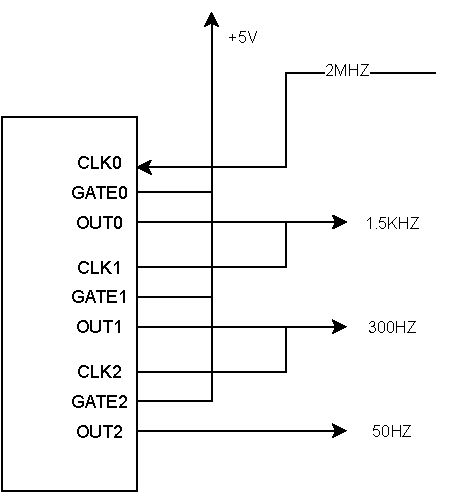
\includegraphics[width=.3\textwidth]{5-1.drawio.pdf}
    \end{center}
\begin{minted}[]{gas}
mov dx, 306h
mov al, 00111110b
out dx, al
mov dx, 300h
mov ax, 1333 ; 2000 / 1.5
out dx, al
mov al, ah
out dx, al

mov dx, 306h
mov al, 01010100b
out dx, al
mov al, 5 ; 1.5 / 0.3
mov dx, 302h
out dx, al

mov al, 10010110b
mov dx, 306h
out dx, al
mov al, 6 ; 300 / 50
mov dx, 304h
out dx, al
\end{minted}
    \1 某微机系统中,8253的端口首地址为40H,时钟频率5MHz,要求通道0输出方波,使计算机每秒钟产生18.2次中断;通道1每隔15us向8237A提出一次DMA请求;通道2输出频率为2000Hz的方波,使编写8253的初始化程序,并画出有关的硬件连接图
    \begin{center}
        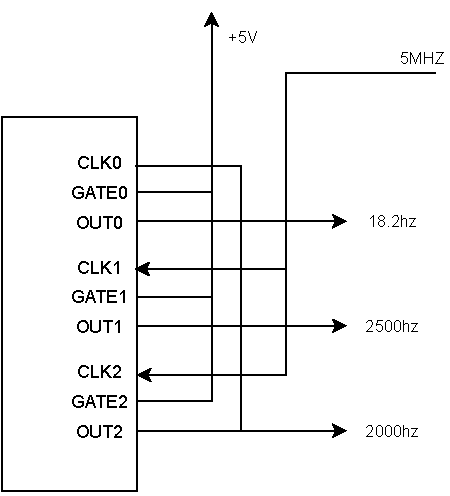
\includegraphics[width=.3\textwidth]{5-2.drawio.pdf}
    \end{center}
    \begin{minted}{gas}
mov dx, 43h
mov al, 10111110b
out dx, al
mov dx, 42h
mov ax, 2500 ; 5000 000 / 2000
out dx, al
mov al, ah
out dx, al

mov dx, 43h
mov al, 00111110b
out dx, al
mov dx, 40h
mov ax, 110 ; 2000 / 18.2
out dx, al
mov al, ah
out dx, al

mov dx, 43h
mov al, 00111110b
out dx, al
mov dx, 41h
mov ax, 2000 ; 5000 000 / 2500
out dx, al
mov al, ah
out dx, al
\end{minted}

\1 设某系统中8254芯片的基地址为F0H,在对3个通道编程时,都设为先读写低8位,后读写高8位,试编程完成下列工作:

    \2 对通道0-2的计数值进行锁存并读出来
\begin{minted}[]{gas}
mov ax, 11011110b
out f3h, al
mov dx, f0h
in al, dx
mov dx, f1h
in al, dx
mov dx, f2h
in al, dx
\end{minted}
    \2 对通道2的状态值进行锁存并读出来
\begin{minted}[]{gas}
mov ax, 11101000b
out f3h, al
mov dx, f3h
in al, dx
\end{minted}
\end{outline}

\end{document}
